\section{Architettura}

\begin{figure}[H]
   \centering
   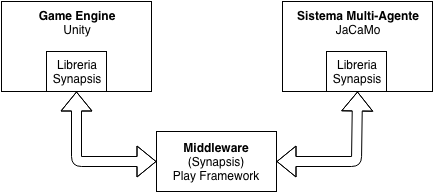
\includegraphics[width=\linewidth]{figures/Architettura_alto_livello.png}
   \caption{Architettura ad alto livello}
\end{figure}

L'immagine mostra la struttura del sistema realizzato per mettere in comunicazione MAS e GE attraverso l'introduzione di un middleware, realizzato con il framework Play, separato e autonomo rispetto alle differenti tecnologie utilzzate su MAS e GE.

\medskip

Per collegare al middleware i due sistemi, sono state realizzate due librerie, definite nell'immagine sovrastante "Libreria Synapsis", contenenti funzionalità di collegamento e comunicazione con Synapsis.
Le librerie rispettano astrazioni e modelli computazionali di entrambi i sistemi (MAS e GE) ed utilizzano la terminologia precedentemente elencata.

\begin{figure}[H]
   \centering
   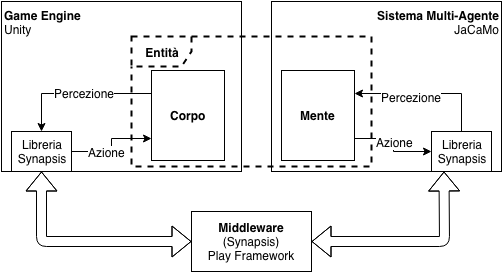
\includegraphics[width=\linewidth]{figures/Middleware_entity.png}
   \caption{Divisione di un'entità nel sistema}
\end{figure}

Aggiungendo un'entità alla struttura precedente è possibile notare come la stessa risulti suddivisa tra i due sistemi (MAS e GE) ed, attraverso il collegamento al middleware, venga reso possibile lo scambio di informazioni (percezioni, azioni) pur essendo computazionalmente separate.